\documentclass{article}
\usepackage{xdi}
\renewcommand{\Summary}{{\xdi} background}

\begin{document}

~

\section*{Use cases for XDI}
\label{sec:background}

\paragraph{Conventional XAS}

In a conventional XAS experiment, we measure a sample somewhere
between 2 and 10,000 scans, possibly requiring dead-time or other
corrections.  Some data processing is required to correct, calibrate,
and/or align the data.  Those scans are then merged into a single
spectrum.

\begin{figure}[h]
  \centering
  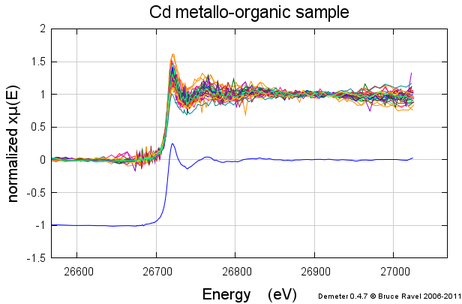
\includegraphics[width=0.5\linewidth]{convxas.png}
  \caption{The merge of several dozen scans at the Cd K edge on a sample dilute in Cd.}
  \label{fig:convxas}
\end{figure}

{\xdi} is about how we express the merged spectrum.

\paragraph{XRF imaging experiments}

In an imaging experiments the heterogeneity of our samples is
measured. XAS can be measured on particular spots.  In this
example\footnote{Tappero et al, New Phytologist 175:4, 641-654, (2007)
  \href{http://dx.doi.org/10.1111/j.1469-8137.2007.02134.x}
  {doi:10.1111/j.1469-8137.2007.02134.x}}, the Co and Ca distribution
in leaf of a metal accumulating plant is shown.  Co micro-XAS spectra
are measured at two spots on the leaf.

\begin{figure}[h]
  \centering
  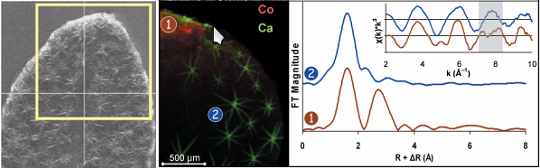
\includegraphics[width=0.7\linewidth]{xrfxas.png}
  \caption{Co K edge micro-XAS measured at two spots on a leaf.}
  \label{fig:xrf}
\end{figure}

{\xdi} is about how we express the micro-XAS spectrum extracted from
the imaging experiment.

\paragraph{Difraction anomalous fine structure (DAFS)}

An anomalous scattering experiments yields energy-dependent scattering
intensities.  Here we see\footnote{Ravel et al. PRB 60, 778-785 (1999)
  \href{http://dx.doi.org/10.1103/PhysRevB.60.778}{doi:10.1103/PhysRevB.60.778}}
DAFS data measured near the Ti K and Ba L$_{\mathrm{III}}$ edges on
BaTiO$_3$.  From these data, $\mu(E)$ or $\chi(k)$ spectra are
extracted and interpreted as position-selective EXAFS.

\begin{figure}[h]
  \centering
  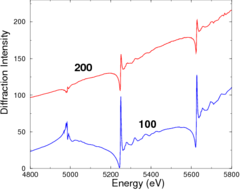
\includegraphics[width=0.3\linewidth]{dafs.png}
  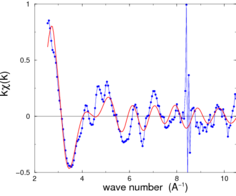
\includegraphics[width=0.3\linewidth]{dafschik.png}
  \caption{A DAFS measurement on BaTiO$_3$.}
  \label{fig:dafs}
\end{figure}

{\xdi} is about how we express the $\mu(E)$ or $\chi(k)$ spectra
extracted from the anomalous diffraction measurement.


\paragraph{Non-resonant inelastic scattering}

A NIXS experiment can used to measure a XANES spectrum in an X-ray
energy loss channel.  Here we see a XANES-like spectrum for graphite
in the X-ray Raman channel, superposed over the Comptopn
scattering.\footnote{Bergmann, et al. Chem. Phys. Lett. 369 184 (2003)
  \href{http://dx.doi.org/10.1016/S0009-2614(02)02003-1}{doi:10.1016/S0009-2614(02)02003-1}}

\begin{figure}[h]
  \centering
  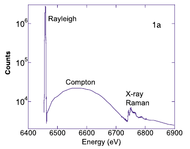
\includegraphics[width=0.2\linewidth]{nixs.png}
  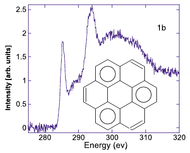
\includegraphics[width=0.2\linewidth]{xels.png}
  \caption{NIXS data measured on graphite.}
  \label{fig:nixs}
\end{figure}

{\xdi} is about how we express the $\mu(E)$ spectra extracted from the
non-resonant inelastic scattering measurement.

\end{document}

%%% Local Variables:
%%% mode: latex
%%% reftex-mode: t
%%% TeX-PDF-mode: t
%%% flyspell-mode: t
%%% TeX-master: t
%%% End:
